
In this chapter, the new algorithms implemented into COSY Infinity by this work is elaborated upon. First, energy straggling via Landau theory is detailed, including novel corrections. Next, the multiple scattering algorithm (which resembles the G4Beamline algorithm discussed in Section~\ref{sec:g4blscattering}) and its implementation is discussed. Finally, the transverse displacement and temporal displacement algorithms are shown.

\Section{Energy Straggling in COSY} \label{sec:COSYStraggling}\par
For energy loss, COSY uses the Bethe-Bloch equation (Eq. \eqref{eqn:bethebloch}) to find the mean energy loss. This can be done in the transfer map paradigm since average energy loss is a deterministic effect. However, this work is concerned with simulating realistic stochastic fluctuations about the average energy loss. For this reason, this work has implemented Landau theory \cite{landau} to describe the straggling distribution. Landau theory is discussed in detail in Section~\ref{ssc:ICOOLStragglingLandau}. 

\iffalse
Other straggling models which were investigated were
\begin{itemize}
\item{Functionalization}
\item{Urb\'{a}n model \cite{geant4}}
\item{Vavilov theory \cite{vavilov}}
\item{Edgeworth series \cite{edgeworth}}
\item{Convolution method (compound Poisson method) \cite{kellerer}}
\item{Landau/Gaussian convolution \cite{hancock}}
\item{Blunck-Liesegang theory \cite{blunck}}
\end{itemize}
However, Landau theory proved to be the best fit. It was chosen over the Vavilov distribution in particular due to a complication where the Vavilov tail was abruptly cut off under certain circumstances.
\fi

Due to its long tail, the average of the Landau distribution is undefined. This is clearly nonphysical. Recall from Eq. \eqref{eqn:landauParameter} that the universal Landau parameter is
\begin{align*}
\lambda=\frac{\epsilon-\left<\epsilon\right>}{\xi}-(1-C_{Euler})-\beta ^2 -\ln (\xi/T_{max}),
\end{align*}
where $\epsilon$ is the energy loss, $C_{Euler}$ is the Euler constant ($\approx 0.577$), $\beta=v/c$ is the relativistic velocity, and $T_{max}$ is the maximum maximum transferrable energy from an incident muon to an electron at rest. However, this means that fluctuations about the mean energy loss $\left(\epsilon-\left<\epsilon\right>\right)$ are also divergent given enough samples. The possibility of divergence results in a sensitivity to step size since smaller steps effectively produce a large sample size. In order to combat this, an artificial cutoff is given to $\lambda$ such that the average Landau $\epsilon$ is equal to the average Bethe-Bloch energy loss $\left<\epsilon\right>$. That is, it is required that
\begin{align*}
\left<\lambda\right>&=\left<\frac{\epsilon-\left<\epsilon\right>}{\xi}\right>-(1-C_{Euler})-\beta^2-\ln(\xi/T_{max})\\
&=-(1-C_{Euler})-\beta^2-\ln(\xi/T_{max}).
\end{align*}
If this cutoff is $\lambda_{max}$, then $\left<\lambda\right>$ can be calculated by the definition of an average over the range $[0,\lambda_{max}]$:
\begin{align*}
\left<\lambda\right>=\frac{\int_0 ^{\lambda_{max}} \lambda * f(\lambda) d\lambda}{\int_0 ^{\lambda_{max}}f(\lambda) d\lambda}.
\end{align*}
The task then is to numerically find $\lambda_{max}$ such that it satisfies
\begin{align*}
\frac{\int_0 ^{\lambda_{max}} \lambda * f(\lambda) d\lambda}{\int_0 ^{\lambda_{max}}f(\lambda) d\lambda}=-(1-C_{Euler})-\beta^2-\ln(\xi/T_{max}).
\end{align*}
GEANT version 3.21 \cite{geant3.21} suggests the following form for $\lambda_{max}$:
\begin{equation} \label{eqn:landauCutoffsGeant3}
\lambda_{max}=0.60715+1.1934\left<\lambda\right>+(0.67794+0.052382\left<\lambda\right>)\exp[0.94753+0.74442\left<\lambda\right>)]
\end{equation}
(note that GEANT4 does not have a section on the Landau cutoff since the Urb\'{a}n model is used instead). However, a plot of required cutoffs ($\lambda_{max}$) vs. desired means ($\left<\lambda\right>$) was produced independently in this work with muon ionization cooling parameters in mind. The form suggested by GEANT3 (see, e.g., Eq. \eqref{eqn:landauCutoffsGeant3}) was used to fit the plot in Figure~\ref{fig:landau_cutoffs}. The determined form of the function is
\begin{equation}\label{eqn:landauCutoffs}
\lambda_{max}=0.517891+1.17765\left<\lambda\right>+(0.476074+0.00880733\left<\lambda\right>)\exp[1.15467+0.984008\left<\lambda\right>].
\end{equation}

\begin{figure}
  \centering
    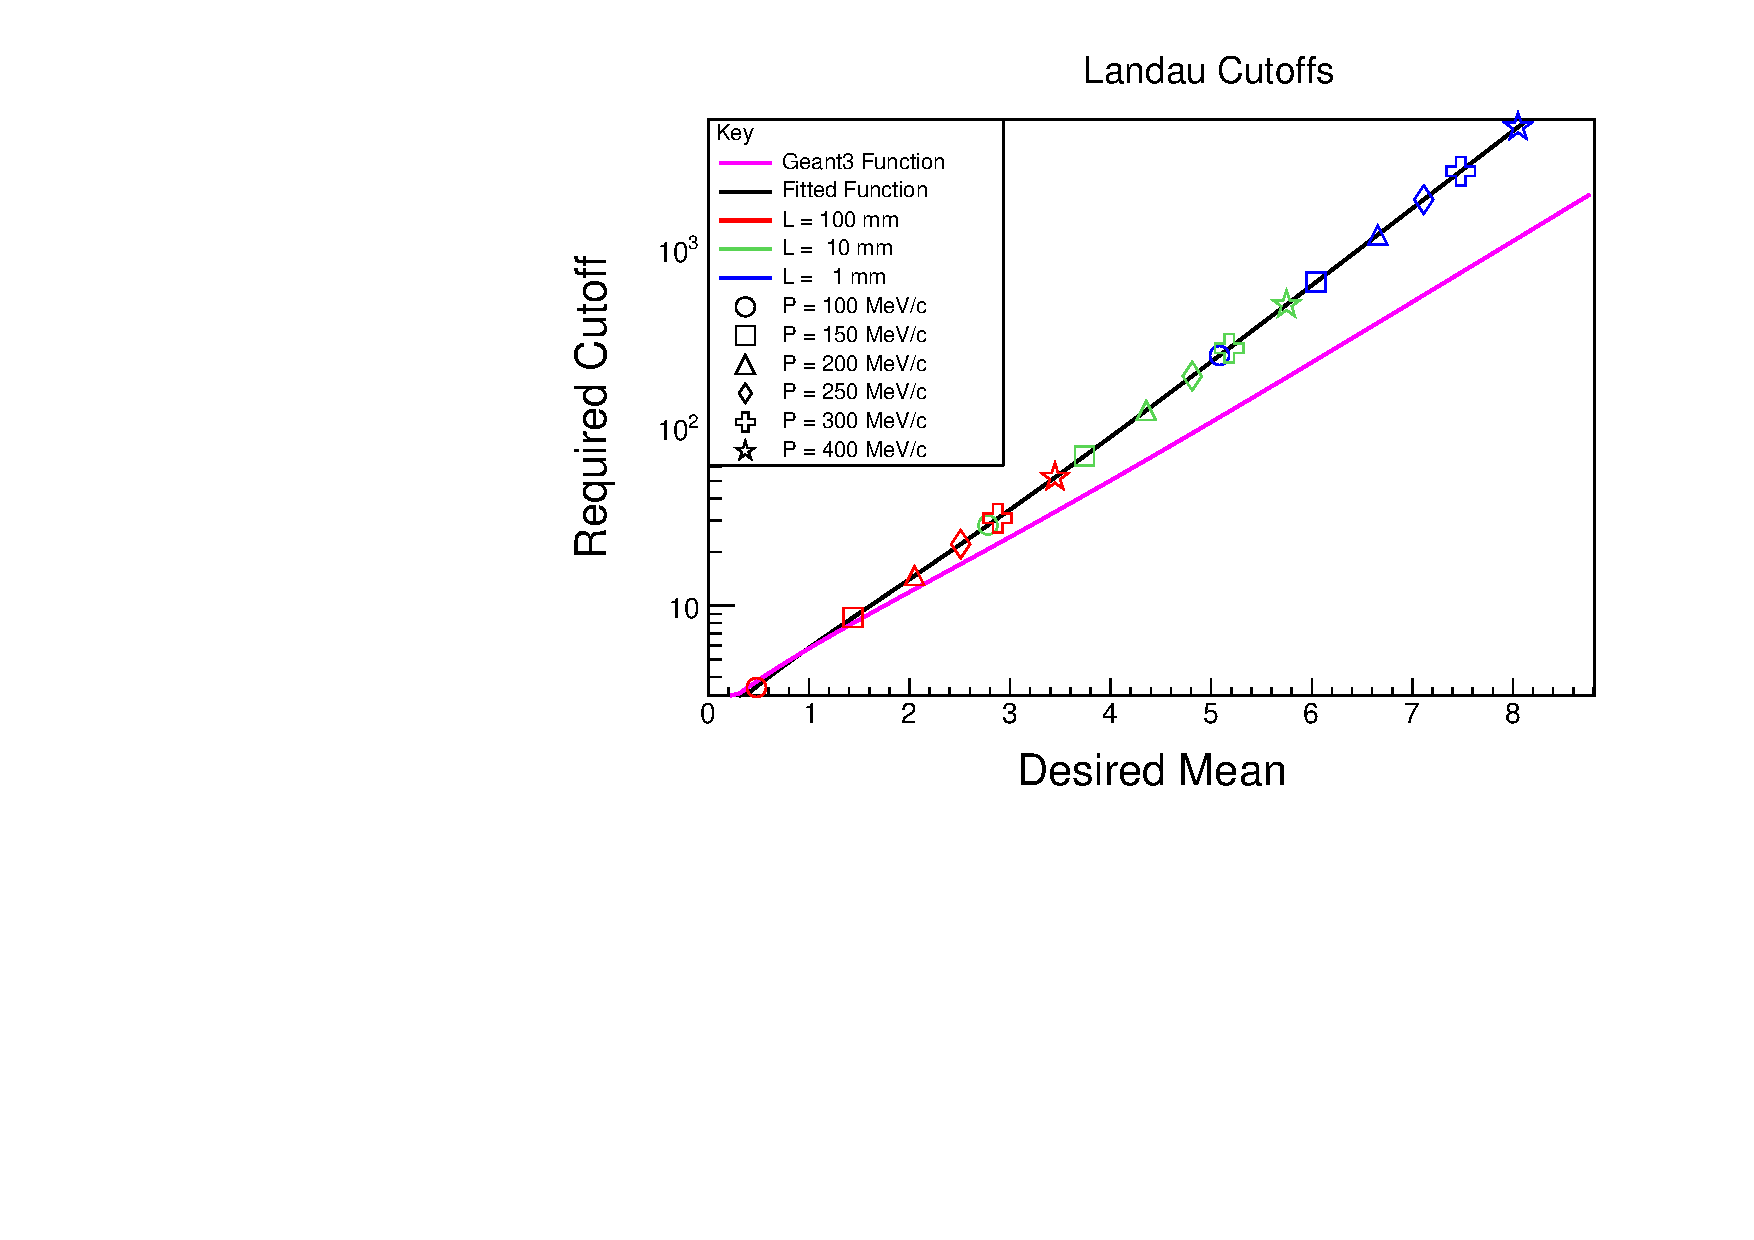
\includegraphics[width=\textwidth]{Figures/landau_cutoffs} 
  \caption[$\lambda_{max}$ vs. $\left<\lambda\right>$ over a variety of liquid hydrogen absorber lengths and initial beam momenta.]{$\lambda_{max}$ vs. $\left<\lambda\right>$ over a variety of liquid hydrogen absorber lengths and initial beam momenta. The pink line is the form given by GEANT3 (see Eq. \eqref{eqn:landauCutoffsGeant3}) and the black line is the fitted curve (see Eq. \eqref{eqn:landauCutoffs}). The data points are combinations of shapes and colors, as seen in the key. For example, since green means 10 mm and the square means 150 MeV/$c$, the green square data point represents the required cutoff for 150 MeV/$c$ muons passing through 10 mm of liquid hydrogen. Liquid hydrogen was chosen in order to match the results in Section~\ref{sec:benchmark}. However, other materials (such as lithium hydride) still fall within the desired $\left<\lambda\right>$ range of [0, 9].}
  \label{fig:landau_cutoffs}
\end{figure}

Based on Eq. \eqref{eqn:landauParameter}, it is possible to find $\epsilon_{max}$:
\begin{align*}
\epsilon_{max}=\xi[\lambda_{max}+(1-C_{Euler})+\beta^2+\ln(\xi/T_{max})]+\left<\epsilon\right>.
\end{align*}
Therefore, during the energy loss sampling, if any energy loss $\epsilon$ is selected which is greater than $\epsilon_{max}$ it is discarded and the sampling is performed again. However, if the result has been discarded 100 times, the particle is assumed to have lost too much energy and is considered lost.

%
%-------------------------------------------------------------------------------
%
\Section{Multiple Scattering in COSY Infinity} \label{sec:COSYScattering}\par
Similar to ICOOL's fifth method of scattering, the Rutherford model (see Section~\ref{sec:ICOOLScattering}), COSY utilizes a piecewise distribution function which is Gaussian  at small angles (as Goudsmit and Saunderson suggested \cite{gs}) and Rutherford-like at large angles. This Rutherford-like tail is derived at length in Appendix~\ref{apx:cosy_cross_section}, with a review of the relevant particle physics symbols and methods in Appendix~\ref{apx:particlePhysicsReview}. The result is the (differential) Mott scattering cross section:
\begin{equation}\label{eqn:MottCrossSection}
\frac{d\sigma}{d\Omega} \propto \frac{1+\frac{(\beta\gamma)^2}{2} (1+\cos\theta)  }{(1-\cos\theta)^2},
\end{equation}
where $d\sigma/d\Omega$ is the differential scattering cross section, $\beta$ is the relativistic velocity, $\gamma=1/\sqrt{1-\beta^2}$, and $\theta$ is the scattering angle. Observe that for the non-relativistic limit $\beta\rightarrow 0$ the cross section does indeed approach a Rutherford distribution (Eq. \eqref{eqn:rutherford}). The practical implementation of this cross section into the probability distribution function is discussed in Section~\ref{ssc:COSYScatteringImplementation}.

\Subsection{Implementation}\label{ssc:COSYScatteringImplementation} Now that the forms of the Gaussian and Rutherford-like scattering cross sections have been obtained, implementation of these cross sections is discussed. In this work, when a particle passes through matter, the change in angle of this particle is selected from a probability distribution. For $u=\cos\theta$, this distribution should be Gaussian-like at small angles \cite{gs} and follow the Mott cross section at large angles. Based on a Gaussian-like cross section for small angles and the cross section in Eq. \eqref{eqn:MottCrossSection}, the distribution has been chosen as
\begin{align}\label{eqn:cosyg}
g(u)=	\begin{cases}
	e^{-a(1-u)} & \quad u_0 \leq u \\
	\zeta\frac{1+\frac{1}{2}(\beta\gamma)^2(1+u-b_c)}{(1-u+b_c)^2} & \quad u\leq u_0
	\end{cases},
\end{align}
where $u_0$ is the cutoff between the Gaussian-like distribution and the Mott distribution, $\zeta$ is the amplitude of the Mott distribution, and $b_c$ is the relative $u$ shift of the Mott distribution. The parameter $a$ is an empirical parameter, based off Highland theory \cite{highland}, and can be found in Eq. \eqref{eqn:geanta}. Eq. \eqref{eqn:geanta} is reproduced here for convenience:
\begin{align*}
a=\frac{0.5}{1-\cos\theta_0}.
\end{align*}
where $\theta_0$ has the form \cite{highland} 
\begin{align*}
\theta_0 = \frac{E_s}{p\beta} \sqrt{\frac{L}{X_0}}.
\end{align*}
However, this definition has been extended in this work to include empirical corrections based on GEANT4's \cite{geant4} treatment of $\theta_0$ (see Eq. \eqref{g4bltheta0}):
\begin{equation}\label{eqn:cosytheta0}
\theta_0 = \frac{13.6 \text{ eV}}{\beta p} \sqrt{\frac{L}{X_0} \Big[ 1+h_1 \ln \frac{L}{X_0} + h_2 \Big(\ln \frac{L}{X_0}\Big)^2 \Big] }.
\end{equation}
The Highland correction terms have been chosen novelly in this work as $h_1=0.12$ and $h_2=0.006$. This was done by fitting the curve given by Eq. \eqref{eqn:cosyg} to match the MuScat results \cite{muscat}, the results of which can be found in Section~\ref{sec:validation}. It is important to note that these correction terms are tunable for future data of muons through higher $Z$ material.

$u_0$ is the point at which the Gaussian term meets the Mott tail. This has been chosen empirically as
\begin{equation}\label{eqn:cosyu0}
u_0=1-\frac{4.5}{a}.
\end{equation}
This parameter was fitted alongside the Highland correction terms to match the experimental results in \cite{muscat}.

$\zeta$ and $b_c$ are the angular scattering distribution's amplitude and offset for the tail. These are found by demanding continuity and smoothness at $u_0$:
\begin{align*}
e^{-a(1-u_0)}&=\zeta\frac{1+\frac{1}{2}(\beta\gamma)^2(1+u_0-b_c)}{(1-u_0+b_c)^2},\\
ae^{-a(1-u_0)}&=\zeta\frac{1+\frac{1}{2}(\beta\gamma)^2(1+u_0-b_c)}{(1-u_0+b_c)^2} \Big(\frac{2}{1-u_0+b_c}+\frac{(\beta\gamma)^2}{2+(\beta\gamma)^2(1+u_0-b_c)}\Big).
\end{align*}
Then
\begin{align*}
a=\frac{2}{1-u_0+b_c}+\frac{(\beta\gamma)^2}{2+(\beta\gamma)^2(1+u_0-b_c)}.
\end{align*}
Solving this for $(u_0-b_c)$ yields a quadratic with the solution
\begin{align} \label{eqn:cosybc}
b_c=u_0+\frac{A_2 + \sqrt{A_2 ^2 - 4A_1 A_3}}{2A_1},
\end{align}
with
\begin{align*}
A_1=&-a(\beta\gamma)^2,\\
A_2=&-(\beta\gamma)^2-2a,\\
A_3=&(\beta\gamma)^2(a-3)+2a-4.
\end{align*}
The continuity condition for $g(u_0)$ yields the expression for $\zeta$:
\begin{equation}\label{eqn:cosyzeta}
\zeta=\frac{e^{-a(1-u_0)}(1-u_0+b_c)^2}{1+\frac{1}{2}(\beta\gamma)^2(1+u_0-b)}.
\end{equation}

Now that the distribution function has a concrete form, it is implemented by inverting the cumulative distribution function (CDF).  Let $G(u)$ be the integral of $g(u)$. Then the variable $G$ is uniformly sampled over the region $[0,G_{max}]$. If $G\geq G(u_0) \equiv G_0$ then the Gaussian part of the distribution is used to generate $u$ (i.e. $G(u\geq u_0)$). Otherwise, the tail of the distribution is used. Figure~\ref{fig:scatdist_example} shows $G(u)$ for $L=100$ mm, $p=200$ MeV/$c$, and a radiation length of $X_0 = 8.66$ m (to simulate a liquid hydrogen target).

\begin{figure}
  \centering
    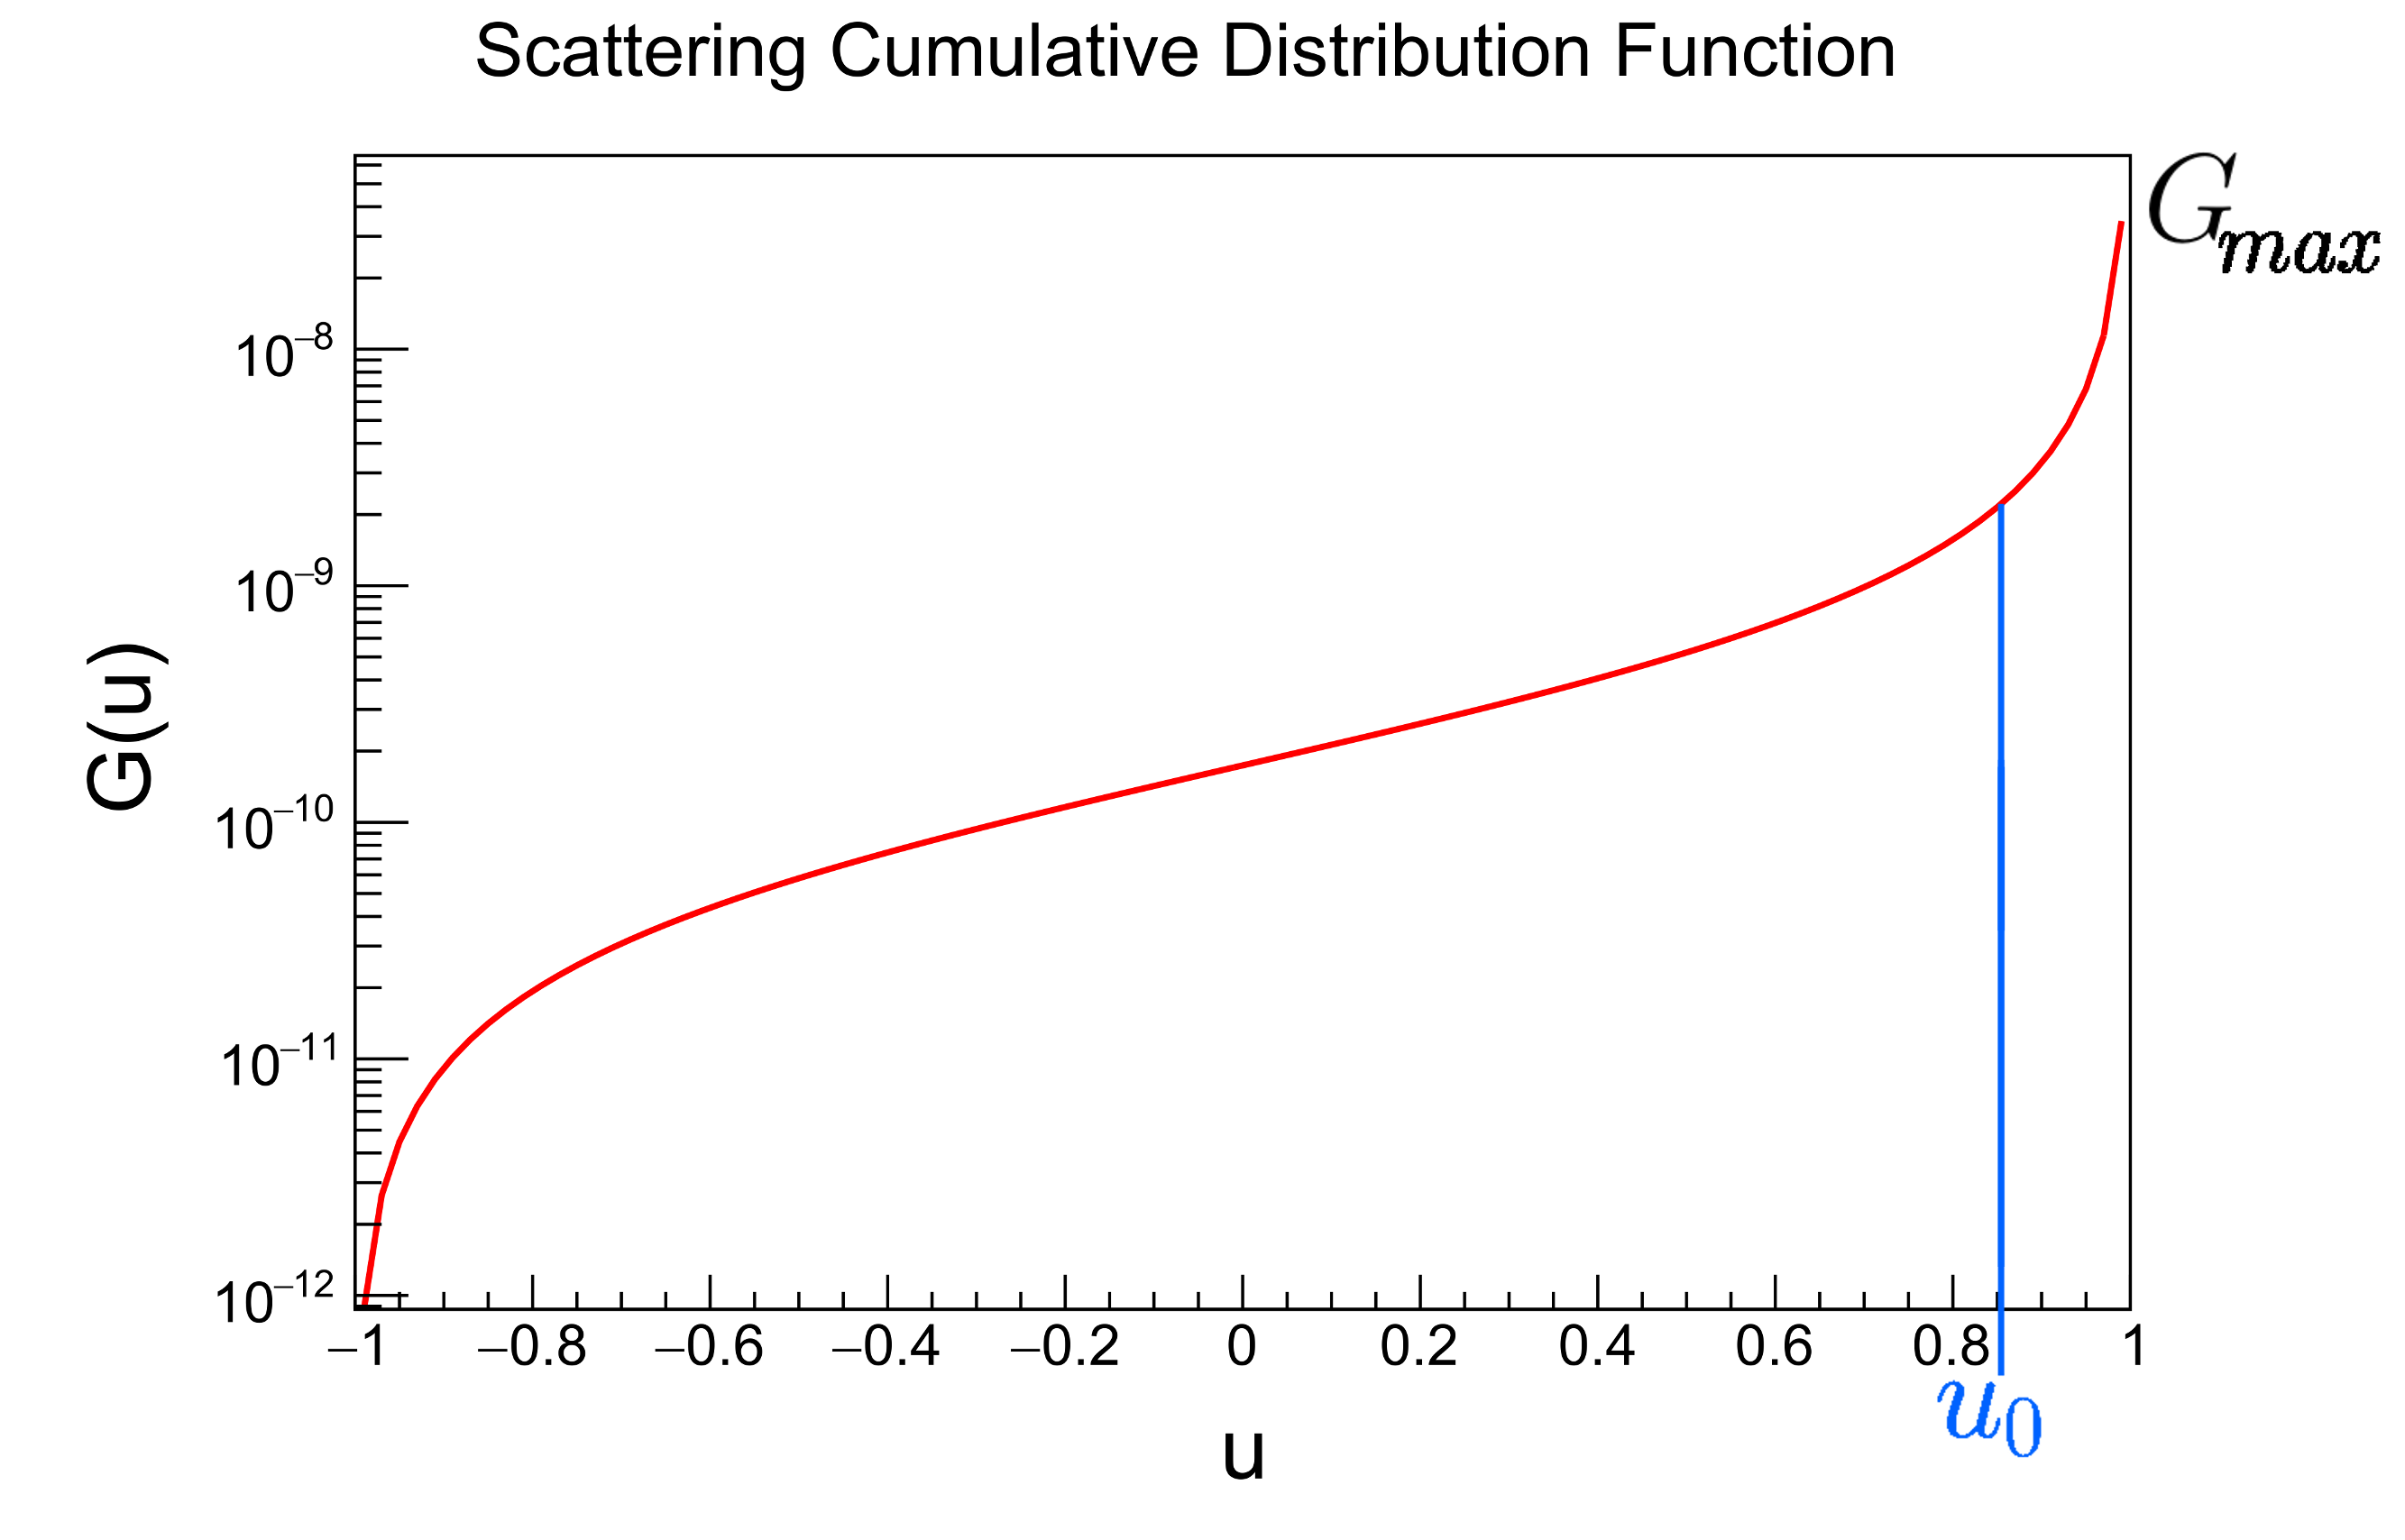
\includegraphics[width=\textwidth]{Figures/scatdist_example} 
  \caption[Example of the COSY cumulative angular distribution function.]{Example of the cumulative angular distribution function for muons with momenta of 200 MeV/$c$ passing through 100 mm of liquid hydrogen. Note that the $y$ axis is log scaled due to the very sharp peak. Furthermore, note that $u_0$ is greatly exaggerated, since its actual value for these parameters is 0.99987.}
  \label{fig:scatdist_example}
\end{figure}

However, since this is a piecewise function, the CDF is inverted in pieces. The tail of the CDF is found first:
\begin{align*}
G(u\leq u_0)=\int _{-1} ^u \zeta \frac{1+\frac{1}{2}(\beta\gamma)^2 (1+u'-b_c)}{(1-u'+b_c)^2} du'.
\end{align*}
This integral may be solved by substituting $v=1-u'+b_c$ and simply splitting the numerator into separate parts:
\begin{align}
\nonumber
G(u\leq u_0)=&-\zeta(1+\frac{1}{2}(\beta\gamma)^2(1-b_c))\int_{2+b_c} ^{1-u+b_c} v^{-2} dv - \\
\nonumber
& \quad \zeta \frac{(\beta\gamma)^2}{2}\int_{2+b_c} ^{1-u+b_c} (v^{-2} - v^{-1} + b_c v^{-2}) dv,\\
G(u\leq u_0)=&\zeta(1+(\beta\gamma)^2)\left(\frac{1}{1-u+b_c} - \frac{1}{2+b_c}\right)+\zeta \frac{(\beta\gamma)^2}{2} \ln\left(\frac{1-u+b_c}{2+b_c}\right). \label{eqn:cosyGTail}
\end{align}

The goal is to solve Eq. \eqref{eqn:cosyGTail} for $u(G)$. However, using direct inversion is extremely difficult and involves special functions. Therefore, it is more prudent to generate  $u$ via bisection method (see Figure~\ref{fig:scatdist_algorithm}). In this method, the true $G$ is sampled uniformly on the range $[0,G_{max}]$, where $G_{max} \equiv G(1)$. Explicitly, $G_{max}$ is
\begin{align*}
G_{max}\equiv G(1) &=\int_{-1} ^{u_0} \zeta\frac{1+\frac{1}{2}(\beta\gamma)^2(1+u-b_c)}{(1-u+b_c)^2}du+\int_{u_0} ^1 e^{-a(1-u)} du,\\
&= G_0+\frac{1}{a}-\frac{e^{-a(1-u_0)}}{a}.
\end{align*}
If $G < G_0$, then the tail is sampled. A trial $u$ called $\bar{u}$ (as in `average') is selected from some range which is known to contain the actual $u$. The range is described as $[u_{min},u_{max}]$, and $\bar{u}=(u_{min}+u_{max})/2$. 

Initially, the range is chosen as $u_{min}=-1$ and $u_{max}=u_0$ (since that is the largest range on which $G(u \leq u_0)$ is valid and hence $u$ is guaranteed to be in this range). $\bar{G} \equiv G(\bar{u})$ is found using Eq. \eqref{eqn:cosyGTail}, and then the routine is subject to the following conditions:
\begin{align*}
&\text{If } \bar{G}\in [G-\delta G,G+\delta G] &\quad &\text{then } u=\bar{u}\text{, return value.}\\
&\text{If } \bar{G} < G-\delta G &\quad &\text{then } u_{min}=\bar{u} \text{, rerun with new }u_{min}.\\
&\text{If } \bar{G} > G+\delta G &\quad &\text{then } u_{max}=\bar{u} \text{, rerun with new }u_{max}.
\end{align*}
$\delta G$ is a precision, and has been chosen for this work as $\delta G = 10^{-8}$. However, it is conceded that in the future $\delta G$ should be a percentage of $G_{max}$ rather than an absolute number.

\begin{figure}
  \centering
    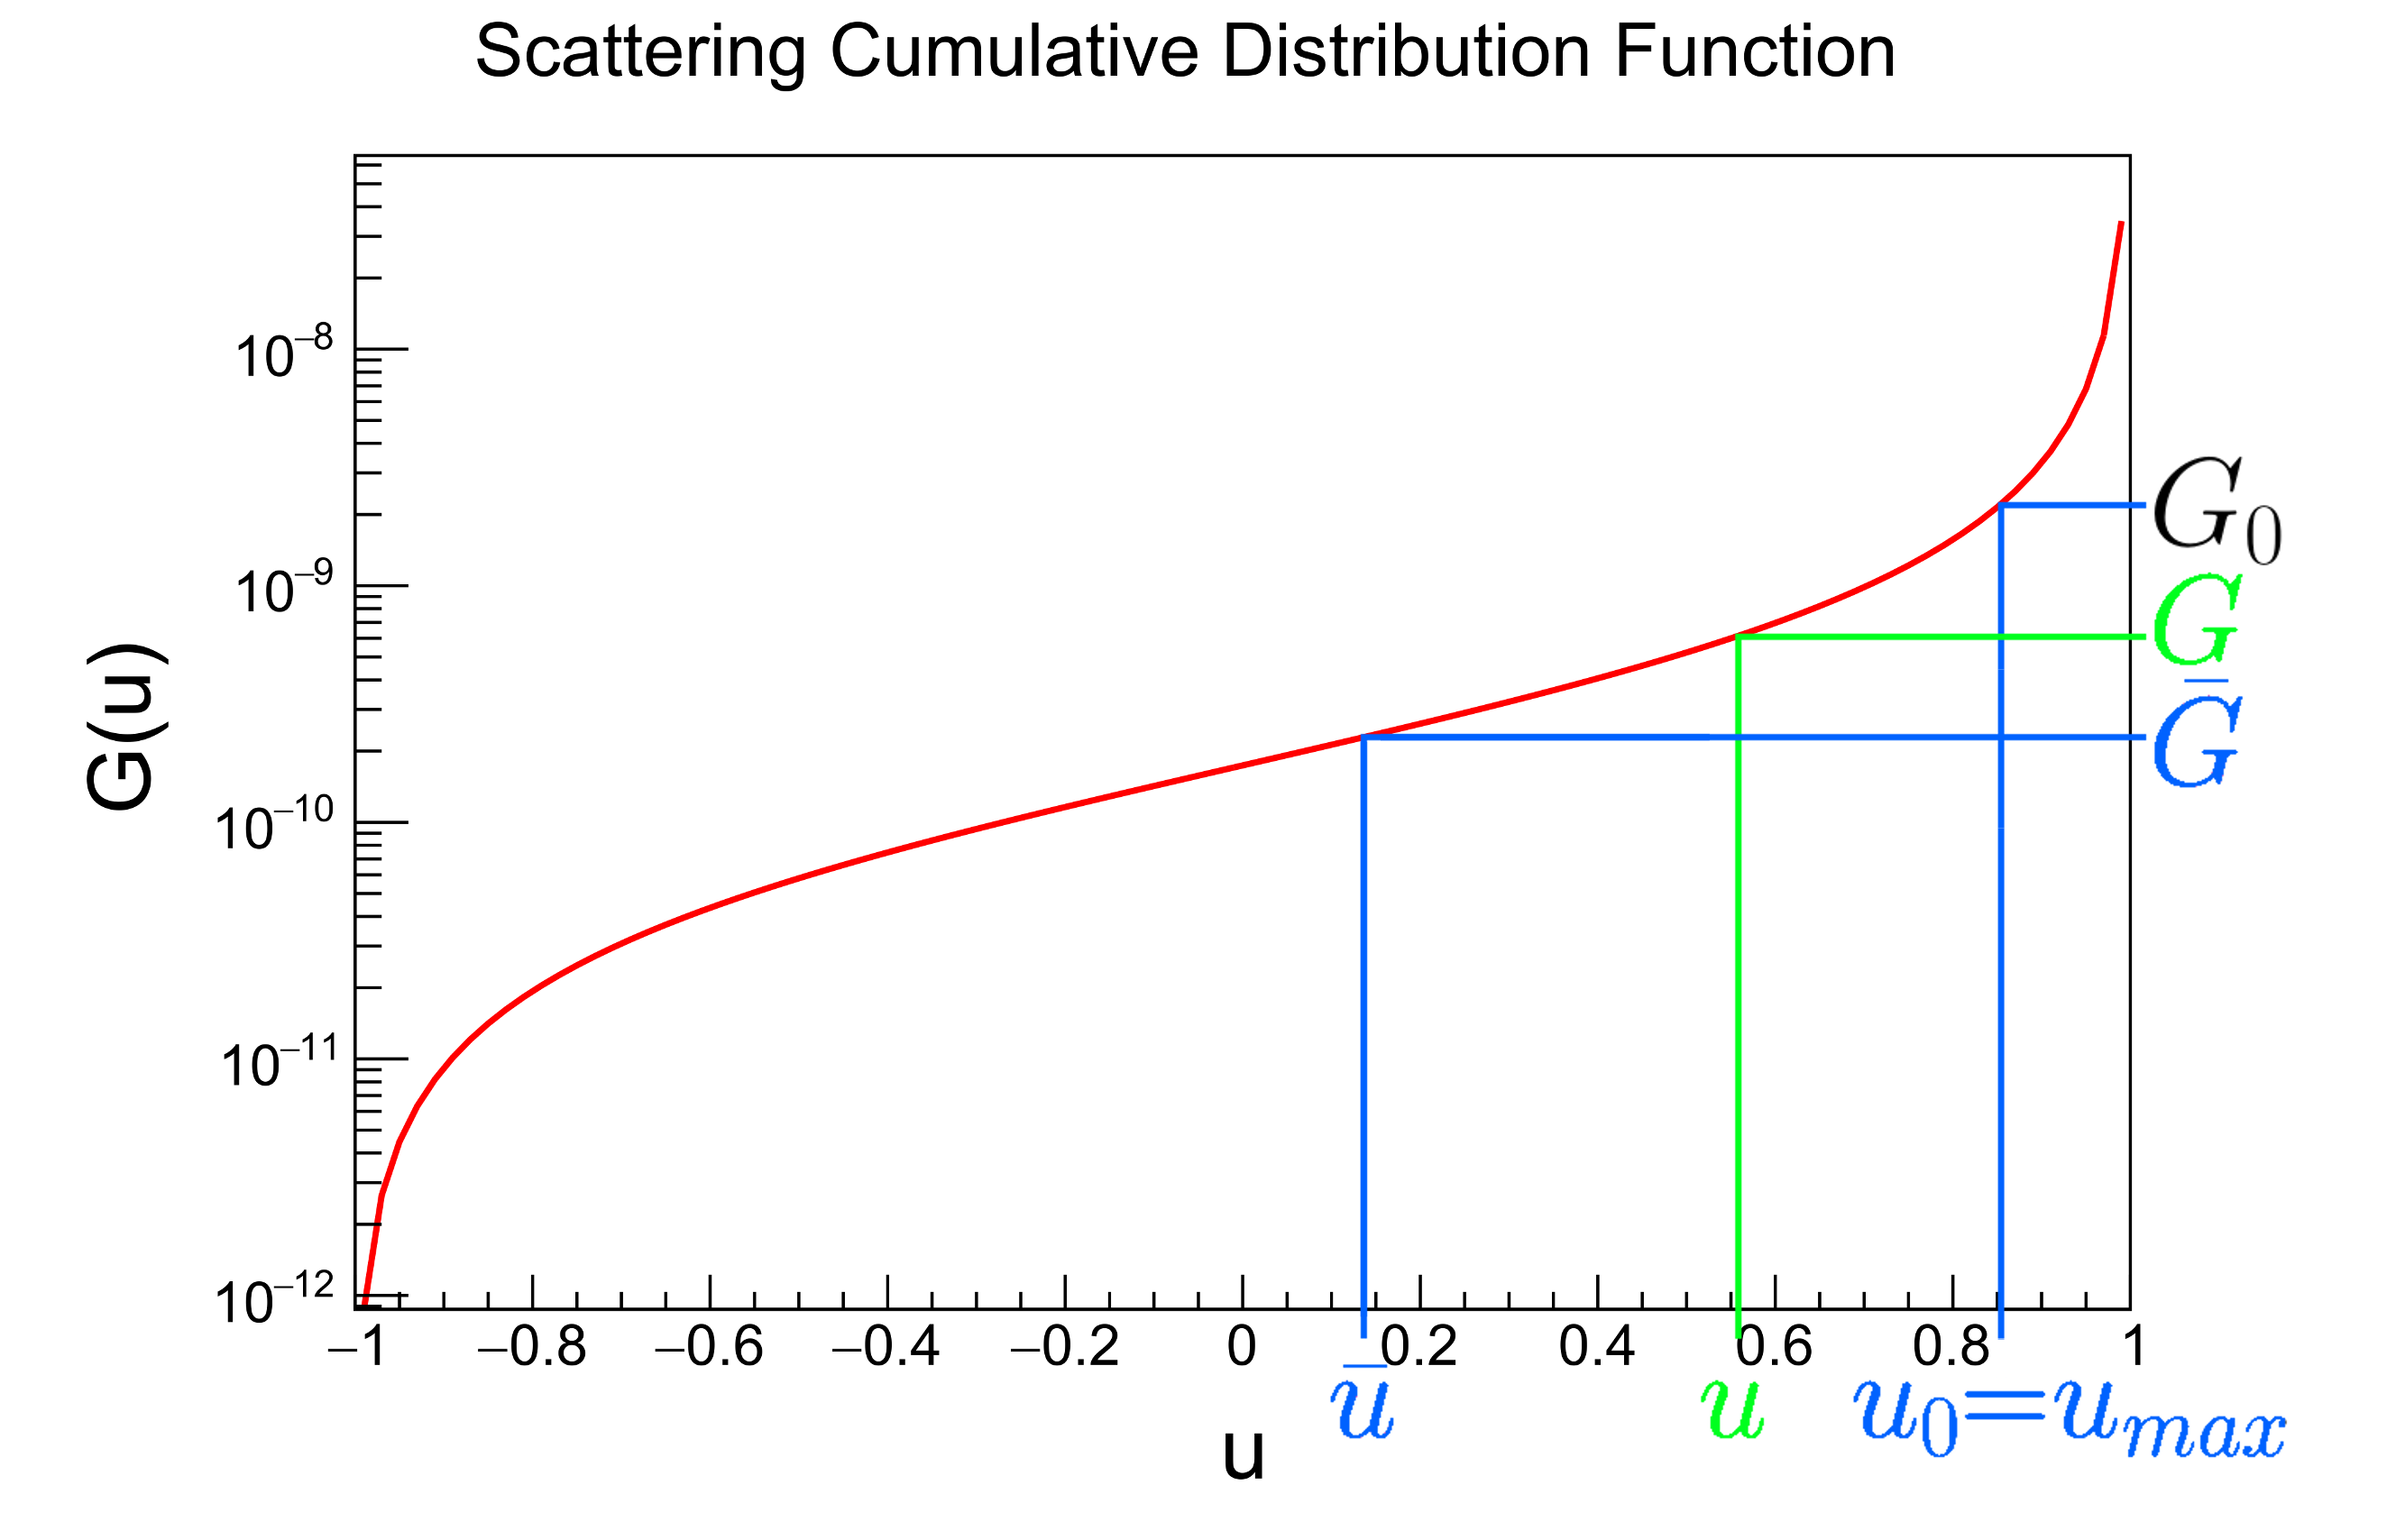
\includegraphics[width=\textwidth]{Figures/scatdist_algorithm} 
  \caption[Example of the first iteration of the COSY CDF algorithm.]{Example of the first iteration of the algorithm to obtain the true $u$ (in green). The true $G$ is chosen uniformly from $G\in[0,G_{max}]$. If $G < G_0$, then the tail is sampled via bisection method. In this case, since $\bar{G} < G$, $\bar{u}$ is the new $u_{min}$ and $\bar{u}$ is calculated again.}
  \label{fig:scatdist_algorithm}
\end{figure}

For the peak, $u_0 \leq u$ and so the CDF becomes
\begin{align*}
G(u_0 \leq u)&=\int_{-1} ^{u_0} g(u) du + \int_{u_0} ^u e^{-a(1-u)} du.
\end{align*}
The first term is simply $G_0$, the cumulative distribution function at $u_0$. The second term is easily integratable and yields
\begin{equation}\label{eqn:cosyGPeak}
G(u_0 \leq u)=G_0 + \frac{e^{-a(1-u)}-e^{-a(1-u_0)}}{a}.
\end{equation}
The inversion of this function is quite straightforward, and is
\begin{equation} \label{eqn:cosyGPeakInverted}
u(G_0 \leq G)=1+\frac{1}{a} \ln \left[a(G-G_0)+e^{-a(1-u_0)}\right].
\end{equation}
Therefore, if $G \in [0,G_{max}]$ is greater than or equal to $G_0$, then it is simply inserted into Eq. \eqref{eqn:cosyGPeakInverted} and the true $u$ is obtained.

It is a subtle yet important point to note that the Mott cross section (Eq. \eqref{eqn:MottCrossSection}), upon which the probability distribution function $g(u)$ in Eq. \eqref{eqn:cosyg} is based, assumes an on-axis straight line trajectory. An on-axis trajectory is equivalent to saying that $p_z=p$ and $x=y=p_x = p_y =0$. For particles that are not on-axis, the reference frame both before and after scattering is rotated such that $p=p_z$. An example of a particle that is not on-axis is exemplified in Figure~\ref{fig:cosyRotatedFrame}. Here, the muon has some angle $\theta_o$ before entering the medium. The lab frame has transverse and longitudinal position axes $T$ and $z$ and the rotated frame has corresponding transverse and longitudinal position axes $T_R$ and $z_R$.  

\begin{figure}
  \centering
    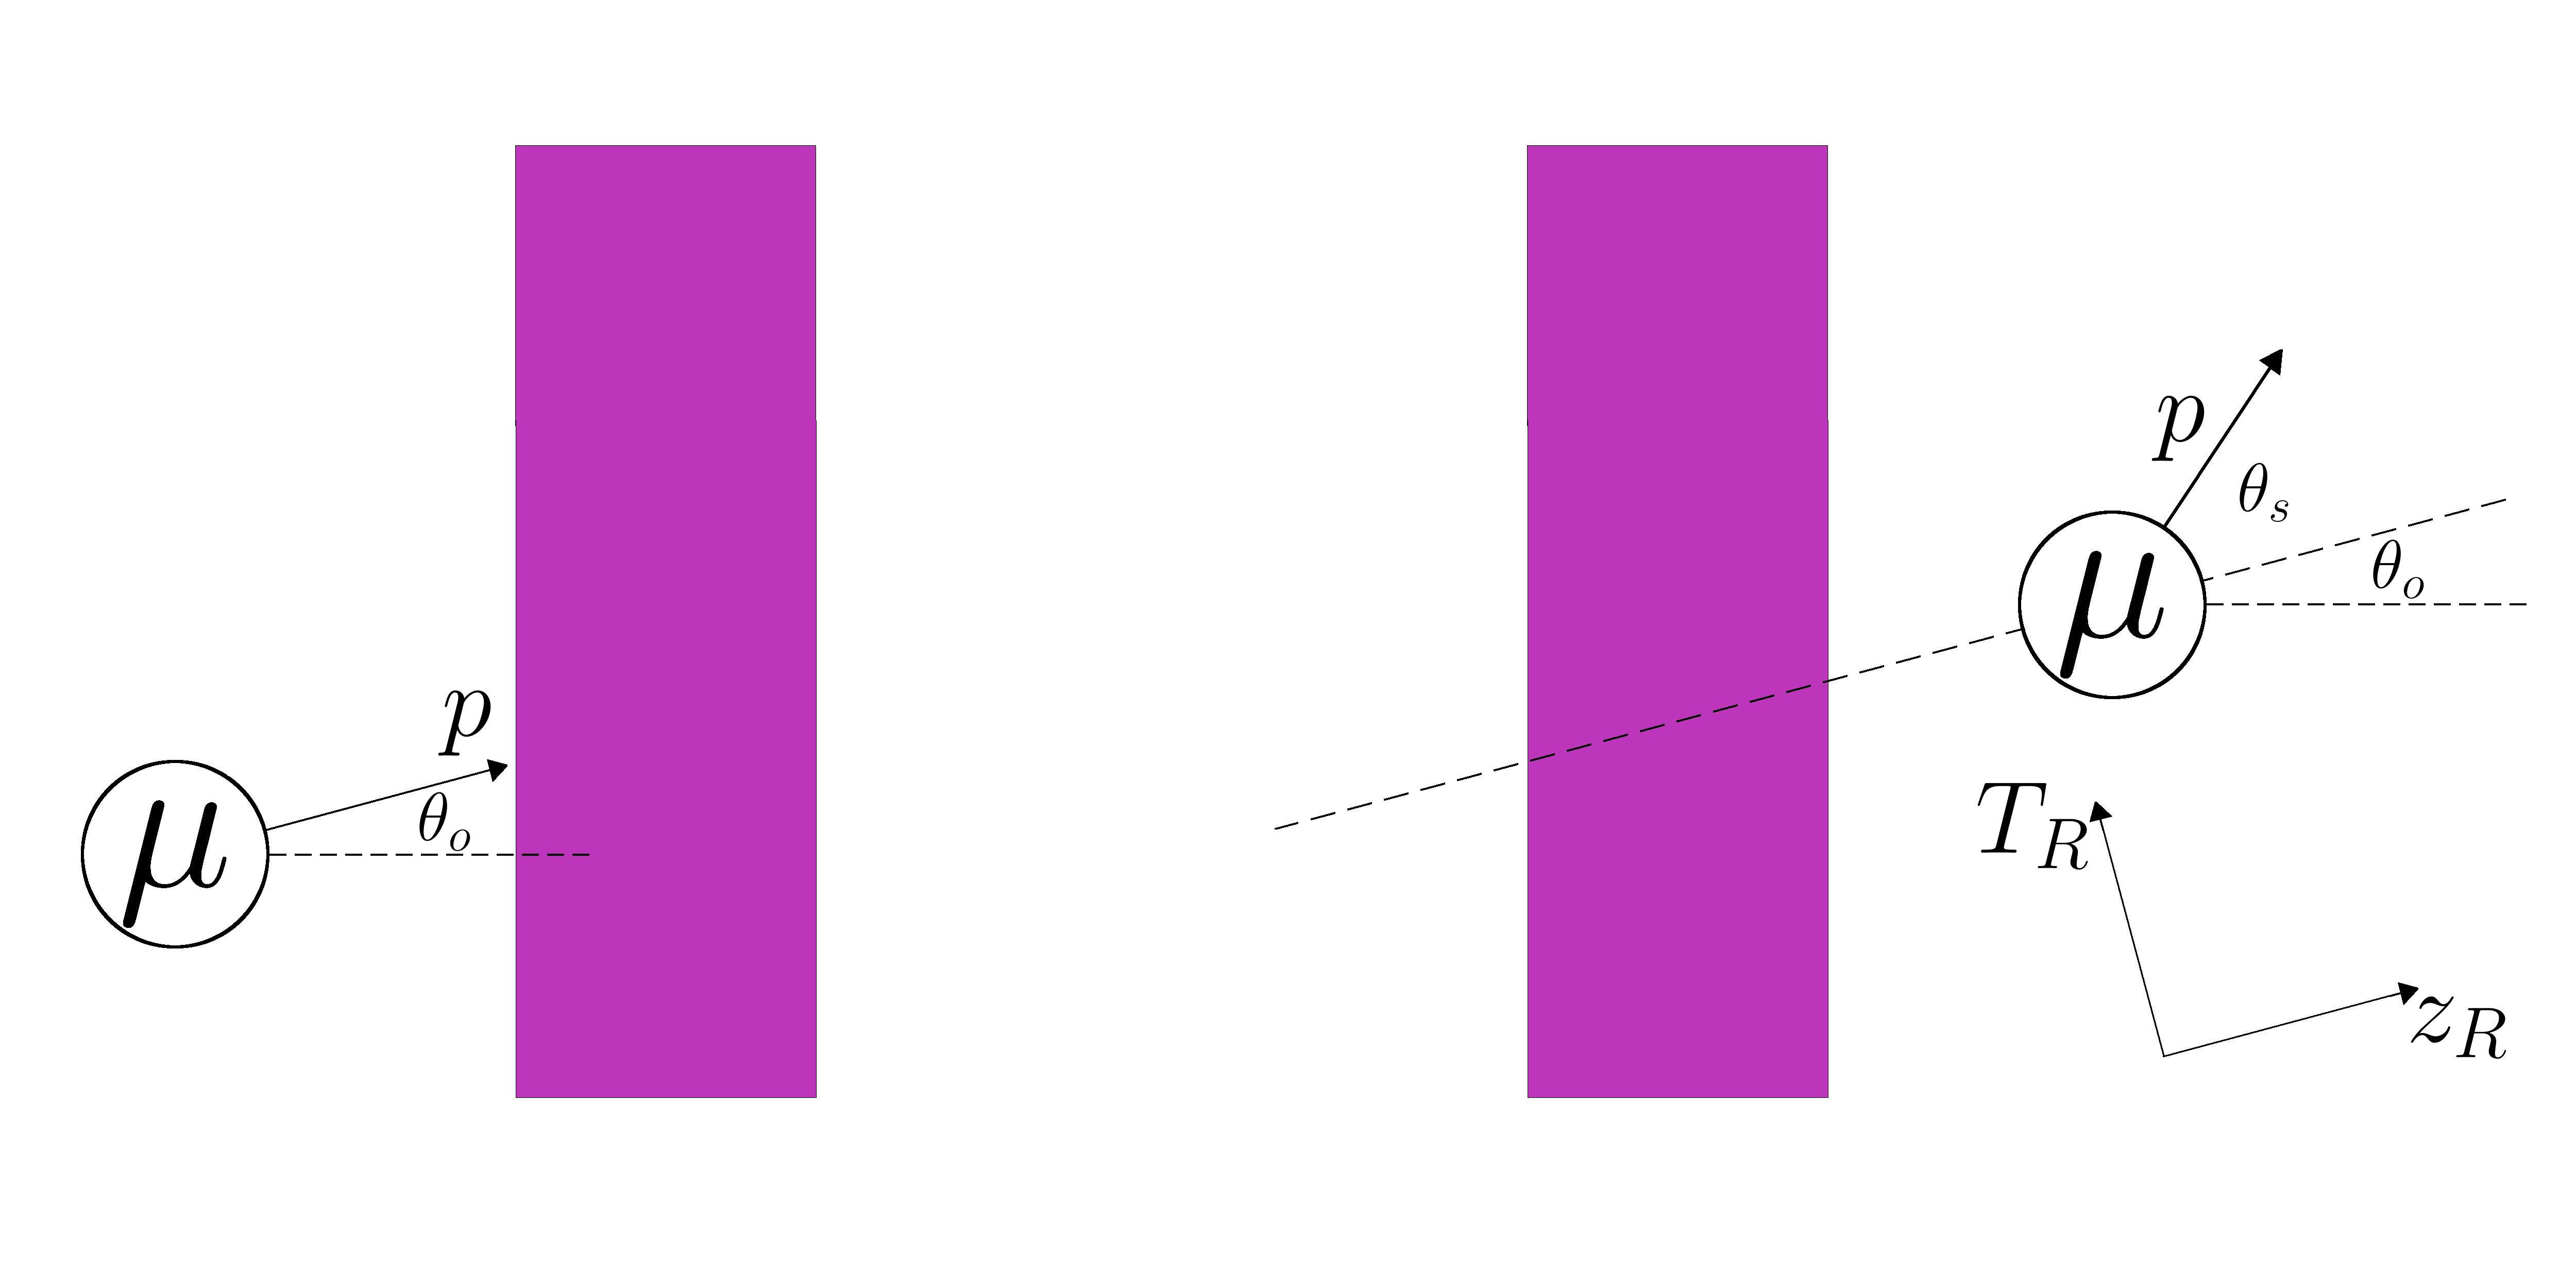
\includegraphics[width=\textwidth]{Figures/cosyRotatedFrame} 
  \caption[Example of a muon entering an absorber with some nonzero initial angle.]{Example of a muon entering an absorber (purple) with some nonzero initial angle $\theta_o$. The muon then scatters an angle $\theta_s$ with respect to its inital momentum $\vec{p}$. The scattering distribution $g(u)$ assumes a straight, on-axis particle ($x=y=p_x=p_y=0$) before scattering, and so is in the rotated frame represented by $T_R, z_R$.}
  \label{fig:cosyRotatedFrame}
\end{figure}

To reiterate, prior to scattering, in the rotated frame the rotated longitudinal momentum is the total momentum ($p_{z,R}=p$) and the rotated transverse momentum is zero ($p_{T,R}=0$). After scattering, $g(u)$ yields the scattered angle $\theta_s$. The rotated longitudinal momentum is no longer necessarily equal to the total momentum, but rather $p_{z,R}=p\cos\theta_s$. Similarly, the rotated transverse momentum is not necessarily zero but instead $p_{T,R}=\sqrt{p^2-p_{z,R}}$. Note that since energy straggling has already been accounted for, the total momentum $p$ stays constant throughout the scattering process and regardless of reference frame.

Due to cylindrical symmetry, the transverse momentum in the rotated frame $p_{T,R}$ must be distributed uniformly into the transverse $x$ and $y$ momenta. The constraint upon the transverse momentum in any frame is
\begin{align*}
p_T^2=p_x ^2+ p_y ^2.
\end{align*}
Therefore, the variable $\phi$ is selected uniformly from [0, 2$\pi$]. The $x$ and $y$ momenta in the rotated frame are
\begin{align*}
p_{x,R}&=P_{T,R}\cos\phi\cdot \text{sgn}(\phi-\pi),\\
p_{y,R}&=P_{T,R}\sin\phi,
\end{align*}
where sgn is the sign function defined by
\begin{align*}
\text{sgn}(x)=	\begin{cases}
		-1 &\qquad \text{for }x<0\\
		\ 0 &\qquad \text{for }x=0\\
		\ 1 &\qquad \text{for }x>0
		\end{cases}.
\end{align*}
The rotated $x$ and $y$ momenta ($p_{x,R}$ and $p_{y,R}$) are subsequently transformed into the lab frame. 
%The process of transforming the rotated scattering into lab coordinates may be found in Appendix~\ref{sec:fortran} on page \pageref{pg:scatdist}.
\iffalse





After energy straggling, the scattering routine which uses $g(u)$ is called.  This routine takes two arguments: $\theta_0$ (the Highland-like critical scattering angle from Eq. \eqref{eqn:cosytheta0}) and $p$, the total momentum. $\theta_0$ includes not only the dependence on material parameters ($L, X_0$) but also dependence on energy terms ($1/\beta p$). $p$ is the total momentum \textit{after} the straggling routine has been called.


The implemented routine for this work that uses the scattering distribution $g(u)$ is called \texttt{SCATDIST}. This routine takes two arguments: $\theta_0$ (the Highland-like critical scattering angle from Eq. \eqref{eqn:cosytheta0}) and $p$, the total momentum. $\theta_0$ includes not only the dependence on material parameters ($L, X_0$) but also dependence on energy terms ($1/\beta p$). $p$ is the momentum \textit{after} the straggling routine has been called. \texttt{SCATDIST} returns not the scattered angle, but the new $z$ momentum $p_z=pu=p\cos\theta$. 

This new $z$ momentum is in the rotated frame, i.e. the frame in which $p_x=p_y=0$ (see Figure~\ref{fig:cosyRotatedFrame}), and so is called $p_{z,R}$. The transverse momentum in the rotated frame, $p_{T,R}$, can be found via $p_{T,R}=\sqrt{p^2-p_{z,R}^2}$. The total transverse angle is $\theta_o + \theta_s$, which includes the original angle ($\theta_o$) and the transverse angle which was gained via scattering ($\theta_s$). Rotation back into the lab frame is given by
\begin{align*}
\begin{pmatrix}
p_{z} \\ p_T
\end{pmatrix}
=
\begin{pmatrix}
\cos\theta_o & -\sin\theta_o\\
\sin\theta_o & \cos\theta_o
\end{pmatrix}
\begin{pmatrix}
p_{z,R} \\ p_{T,R}
\end{pmatrix}.
\end{align*}

\begin{figure}
  \centering
    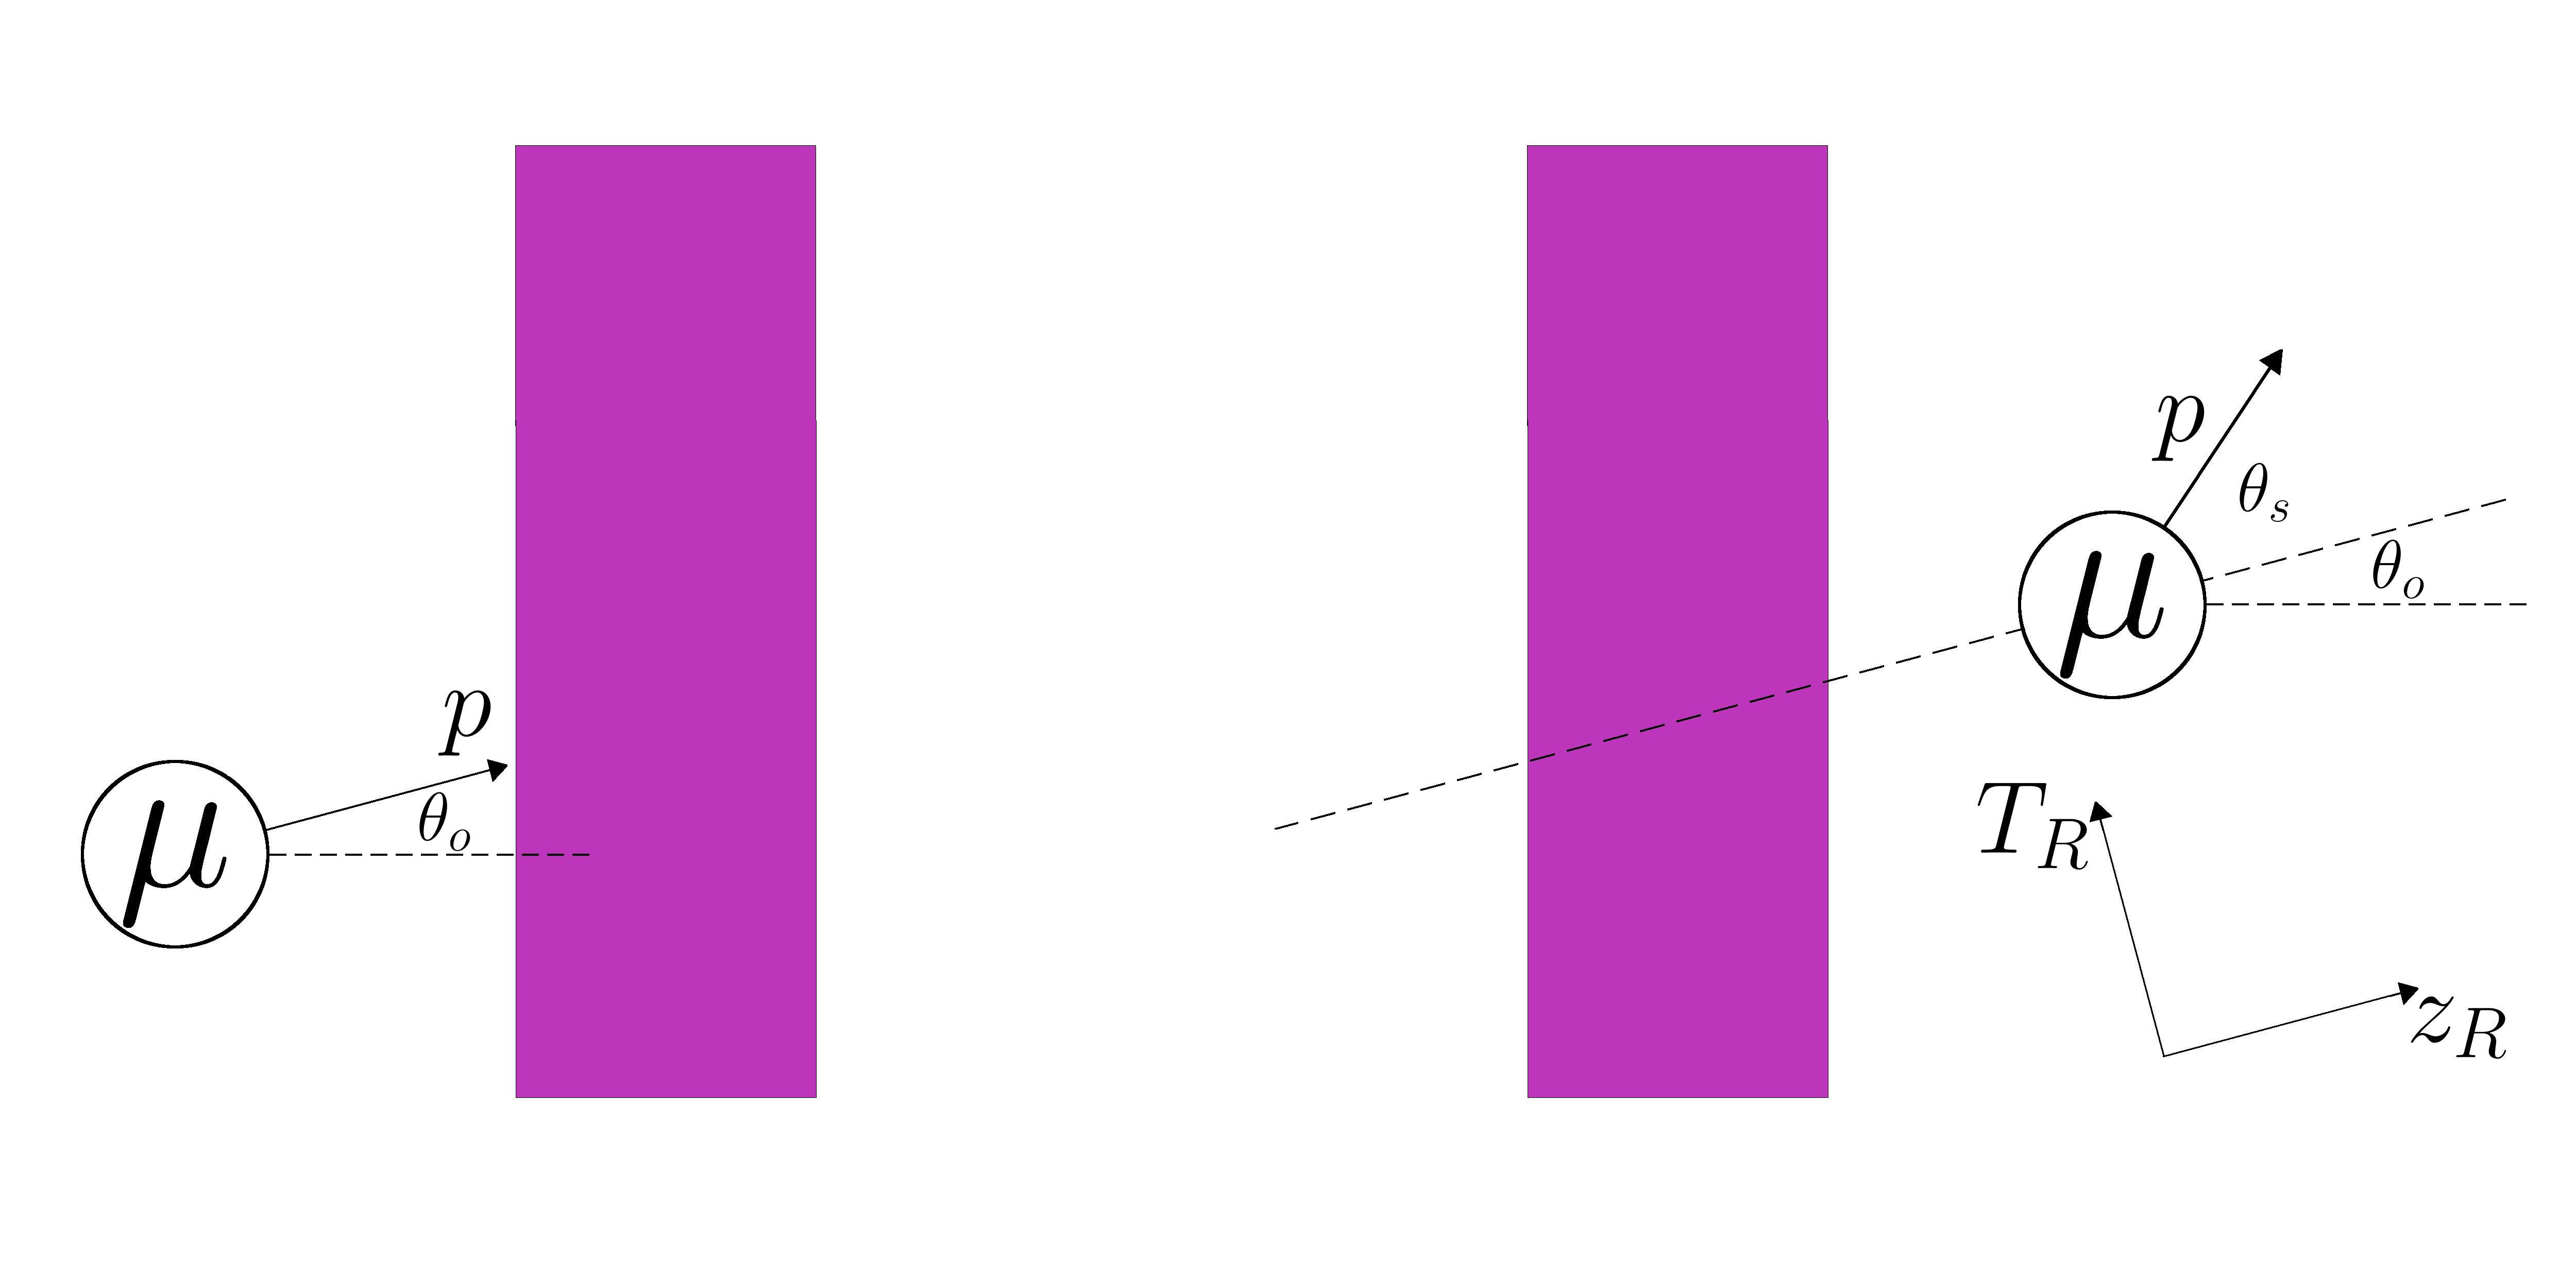
\includegraphics[width=\textwidth]{Figures/cosyRotatedFrame} 
  \caption[Example of a muon entering an absorber with some nonzero initial angle.]{Example of a muon entering an absorber (purple) with some nonzero initial angle $\theta_o$. The muon then scatters an angle $\theta_s$ with respect to its inital momentum $\vec{p}$. The scattering distribution $g(u)$ assumes a straight, on-axis particle ($x=y=p_x=p_y=0$) before scattering, and so is in the rotated frame represented by $T_R, z_R$.}
  \label{fig:cosyRotatedFrame}
\end{figure}

Note that at this point one must not uniformly distribute $p_T$ into $p_x$ and $p_y$. This is because, for example, if $p_x$ was positive before scattering it should have a strong probability of being positive after scattering. If one were to distribute $p_T$ uniformly then $p_x$ would have a 50/50 chance of being negative. For this reason, only the transverse momentum gained via scattering should be uniformly distributed into $p_x$ and $p_y$.

Let the original momenta (after straggling but before scattering) be denoted with the subscript $o$ in the same fashion that $\theta_o$ is the angle before scattering. Then the amount of transverse momentum which was gained via scattering is $P_T-P_{T,o}$. This new amount of transverse momentum must be added to the original $p_{x,o}$ and $p_{y,o}$ uniformly due to cylindrical symmetry. Consequently, let $\phi$ be an angle chosen from $[0,2\pi]$. Then the final $p_x$ and $p_y$ are
\begin{align*}
p_x&=p_{x,o}+(P_T-P_{T,o})\cos\phi\\
p_y&=p_{y,o}+(P_T-P_{T,o})\sin\phi.
\end{align*}







\fi

To summarize, the angular distribution used by COSY Infinity is based on a piecewise function which is Gaussian for small angles \cite{gs} and has a Mott tail for large angles. This distribution is represented by $g(u)$ in Eq. \eqref{eqn:cosyg}, where $u\equiv \cos\theta$. $g(u)$ has four parameters: $a$, an empirical parameter that is based on Highland theory \cite{highland} and is dependent on some critical angle $\theta_0$, defined in Eq. \eqref{eqn:cosytheta0}; $u_0$, the empirical cutoff angle that distinguishes which angles are Gaussian and which are not, found by Eq. \eqref{eqn:cosyu0}; $b_c$, a parameter derivable from smoothness of $g$ at $u_0$, which represents the offset of the Mott tail, found in Eq. \eqref{eqn:cosybc}; and $\zeta$, a parameter derivable from continuity of $g$ at $u_0$ which represents the amplitude of the Mott tail, found in Eq. \eqref{eqn:cosyzeta}. From $g(u)$, its antiderivative $G(u)$ may be found and a particular $G$ may be picked from the range $[0,G_{max}]$. If $G<G_0 \equiv G(u_0)$, then $u$ comes from the Mott tail and a bisection method is used to find $u$. If $G_0 \leq G$ then $u$ comes from the Gaussian peak and $G(u)$ may be inverted to find $u(G)$. This scattered angle must then be rotated into the lab frame and the additional transverse momentum must be uniformly distributed into $p_x$ and $p_y$.

%
%-------------------------------------------------------------------------------
%
\Section{Transverse Displacement in COSY Infinity}\label{sec:COSYTransverseDisplacement}\par
Due to multiple scattering events, when a particle traverses matter, a direct correlation between the particle transverse position and scattered angle is not always clear. Two identical particles with identical initial conditions may end up with identical scattered angles but different transverse positions (see Figure~\ref{fig:lateral_displacement}). This is because these two particles may take different paths through the absorber. While both of these paths may lead to a similar final angle with respect to the $z$ axis, the positions are likely different due to their trajectories.

\begin{figure}
  \centering
    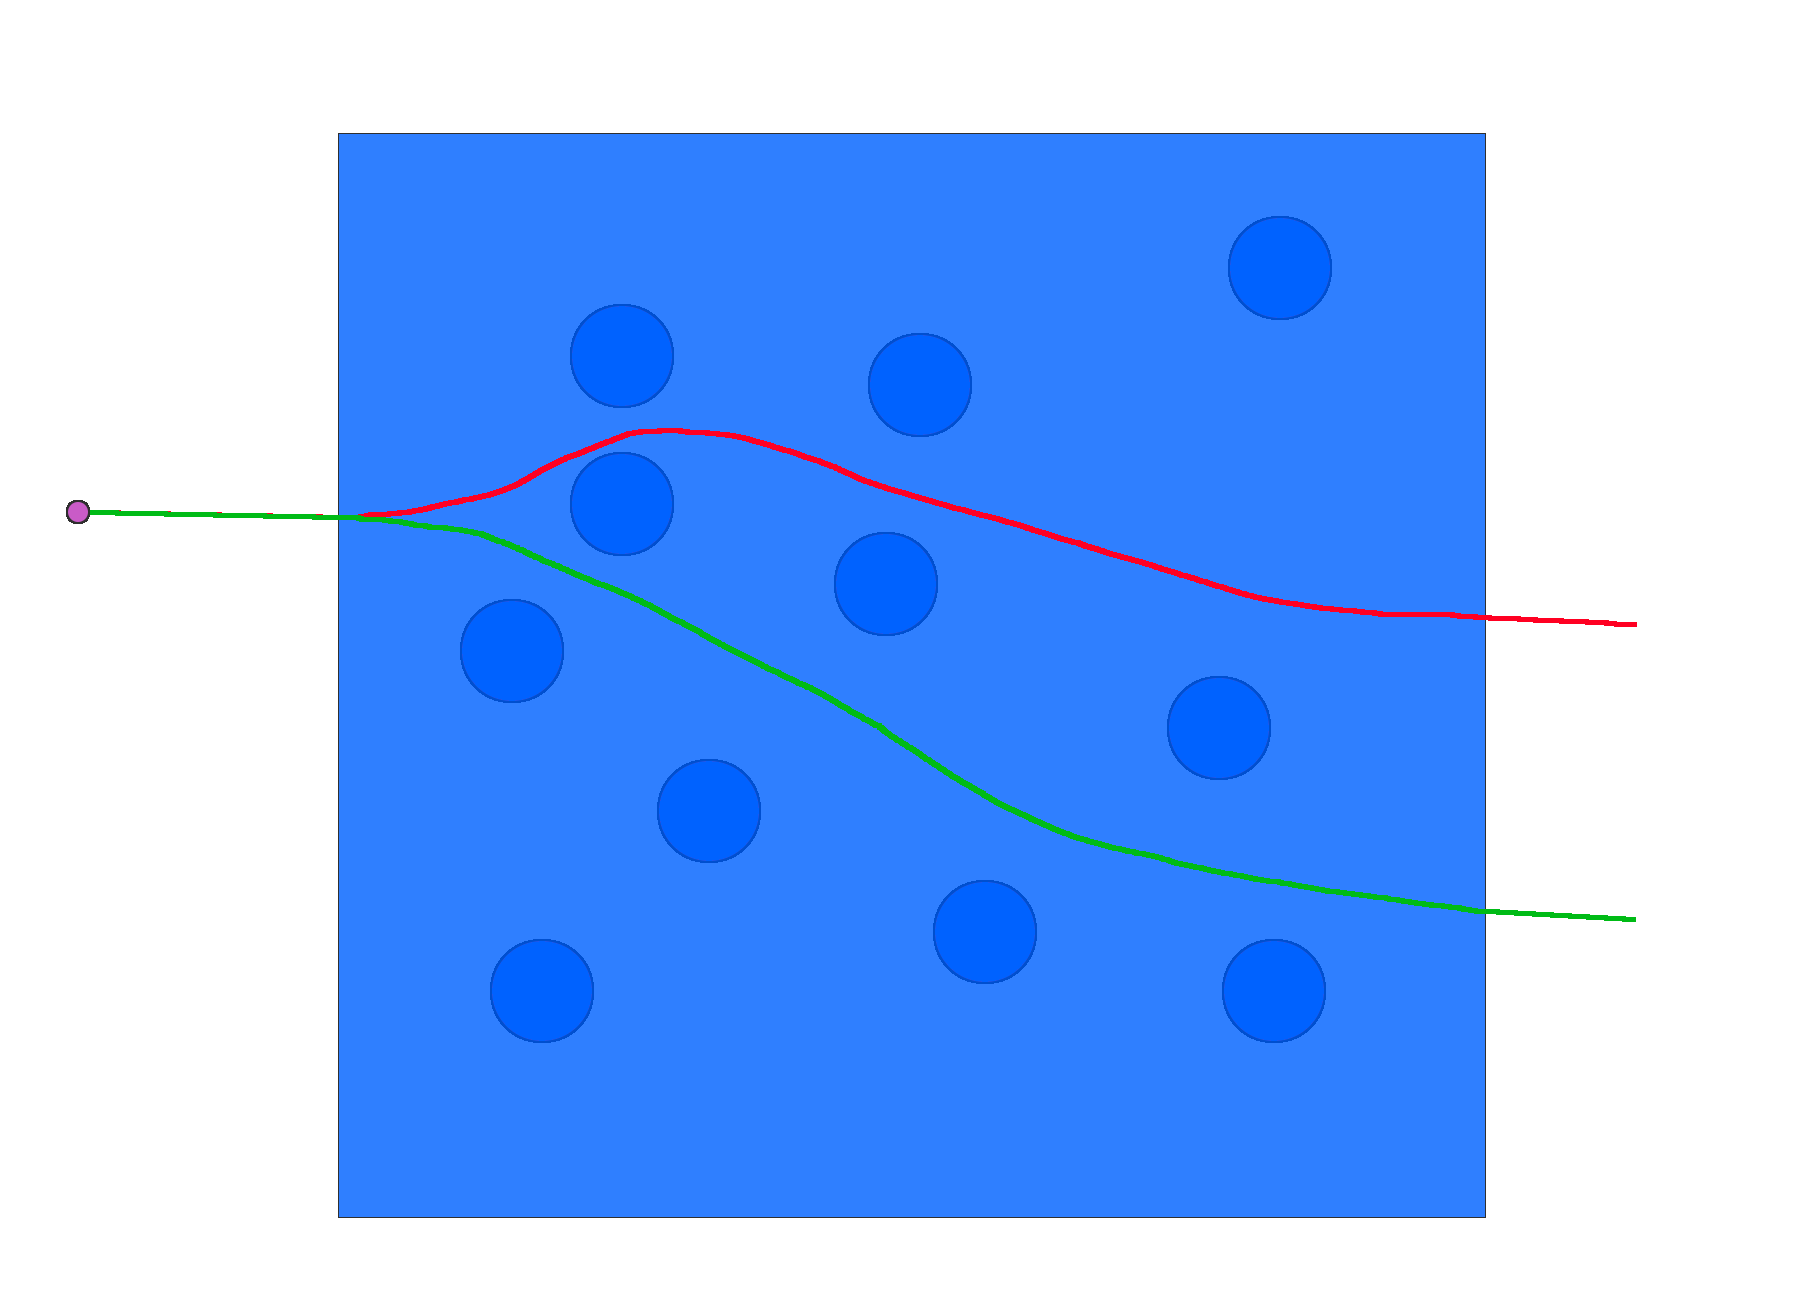
\includegraphics[width=0.75\textwidth]{Figures/lateral_displacement} 
  \caption[Two examples of true paths.]{Two examples of true paths which a particle might take when traversing a medium. Note that both the red and green paths have the same final scattered angle but different transverse positions.}
  \label{fig:lateral_displacement}
\end{figure}

For this reason, transverse corrections have been implemented in  COSY. Due to a lack of experimental data at the time, COSY was compared to G4Beamline across several initial momenta and absorber lengths. The result was
\begin{equation}\label{eqn:cosylatdis}
x = x_o + x_D+\text{Gaus}(\theta_\textit{diff} *L/2,\theta_c /(2\sqrt{3})),
\end{equation}
where $x_o$ is the original $x$ position, $x_D = L*P_{x,o}/P_{z,o}$ is the deterministic  gain in $x$, and Gaus($\mu,\sigma$) is a randomly selected number from a Gaussian distribution with mean $\mu$ and standard deviation $\sigma$. The forms of $\mu$ and $\sigma$ were selected based on a combination of the Particle Data Group \cite{PDG} and Fernow and Gallardo  \cite{fernowAndGallardo}. Note that the average $\mu=\theta_\textit{diff}*L/2$ represents the transverse displacement that would have occured if all of the angular scattering had happened at the point $L/2$. $\theta_\textit{diff}=\theta_\textit{final}-\theta_o$ is the amount of deflection which occurred due to scattering and $\theta_c=13.6 \text{ eV}/\beta p \cdot \sqrt{1/X_0}$ is the coefficient from Highland theory \cite{highland}.

The fitting of these parameters is discussed next. As previously mentioned, the data for the fits were generated by G4Beamline \cite{g4bl}. Here, a particular example of a simulation of $10^6$ particles passing through 1 cm of liquid hydrogen is shown. The initial beam distribution was a pencil beam of momentum 200 MeV/$c$. A plot of the histogram of $(x,p_x)$ phase space can be seen in Figure~\ref{fig:xpx_phase_space}. It can be seen in Figure~\ref{fig:xpx_phase_space_cut} that the cross section of a given transverse momentum results in a nearly-Gaussian $x$ histogram. It can also be inferred from the figure that the mean and standard deviation of the Gaussian fit varies depending on which $p_x$ is chosen. For example, higher values of $p_x$ appear to have both a larger mean and standard deviation. While this trend is conceptual, it aids in the understanding of the form of Eq. \eqref{eqn:cosylatdis}.

The phase space portrait in Figure~\ref{fig:phase_space_portrait} shows that the distribution is only locally Gaussian. However, fitting in the range of $p=100\text{--}400$ MeV/$c$, $L=1\text{--}100$ mm has shown that this is a good approximation for the majority of particles (see Section~\ref{sec:benchmark}).

An example of the success of this implementation can be seen in Figure~\ref{fig:xpx_phase_space_implemented}, where $10^6$ muons of momentum 250 MeV/$c$ were simulated through 100 mm of liquid hydrogen. The simulation was carried out in both COSY and ICOOL \cite{icool} with good agreement.

\begin{figure}[H]
  \centering
    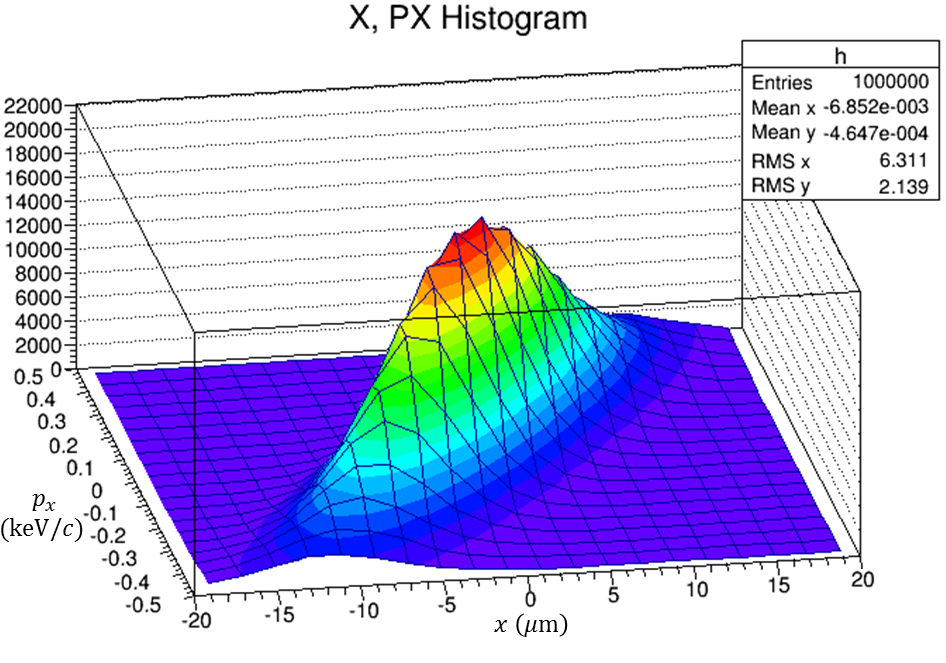
\includegraphics[width=0.7\textwidth]{Figures/xpx_phase_space} 
  \caption[2D histogram of $(x,p_x)$ phase space.]{2D histogram of $(x,p_x)$ phase space for $10^6$ muons of momentum 200 MeV/$c$ passing through 1 cm of liquid hydrogen.}
  \label{fig:xpx_phase_space}
\end{figure}

\begin{figure}[H]
  \centering
    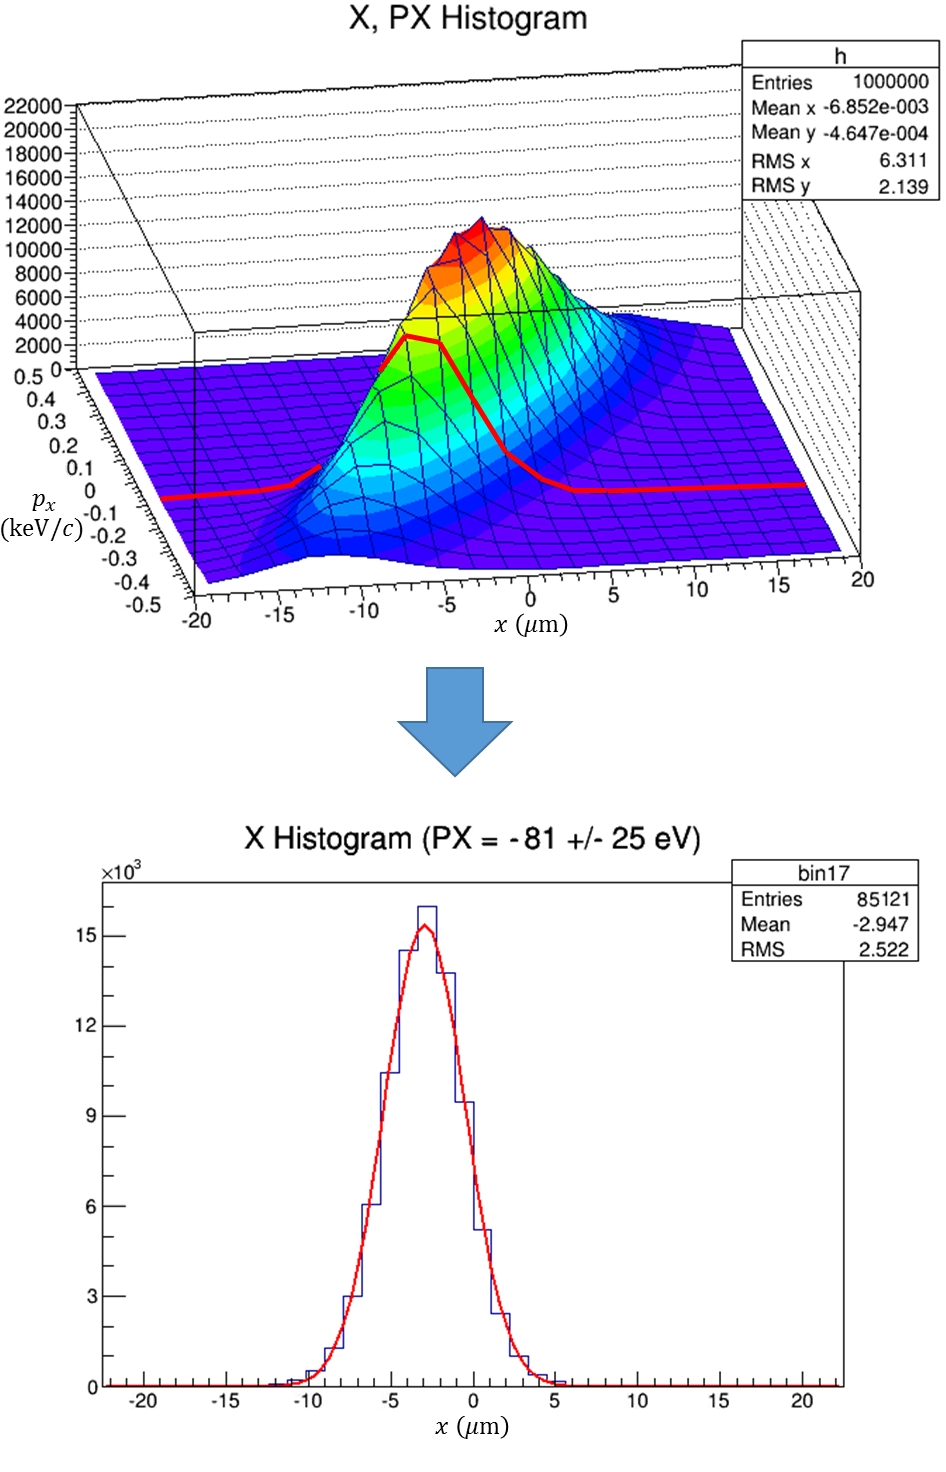
\includegraphics[width=0.7\textwidth]{Figures/xpx_phase_space_cut} 
  \caption[Cross section of Figure~\ref{fig:xpx_phase_space} at $p_x=0.08$ keV/$c$.]{Cross section of Figure~\ref{fig:xpx_phase_space} at $p_x=(-0.081 \pm 0.025)$ keV/$c$. The resulting $x$ histogram fit (in red) is nearly Gaussian.}
  \label{fig:xpx_phase_space_cut}
\end{figure}

\begin{figure}[H]
  \centering
    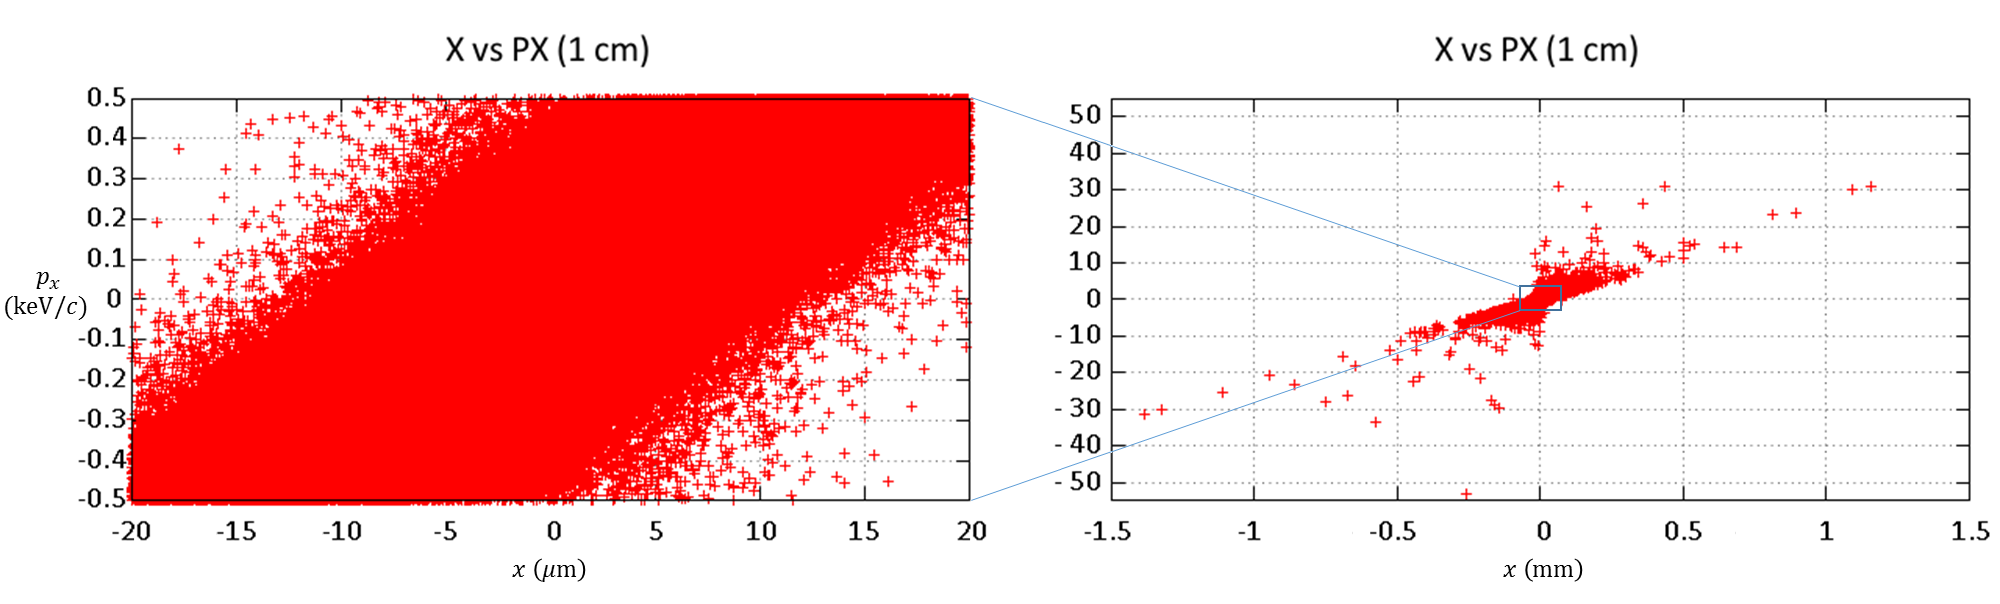
\includegraphics[width=\textwidth]{Figures/phase_space_portrait} 
  \caption[Phase space portrait of Figure~\ref{fig:xpx_phase_space}.]{Phase space portrait of Figure~\ref{fig:xpx_phase_space}. Observe that the bulk in Figure~\ref{fig:xpx_phase_space} is represented on the left. Further observe that the extrema of this distribution do not follow a Gaussian curve.}
  \label{fig:phase_space_portrait}
\end{figure}

\begin{figure}[H]
  \centering
    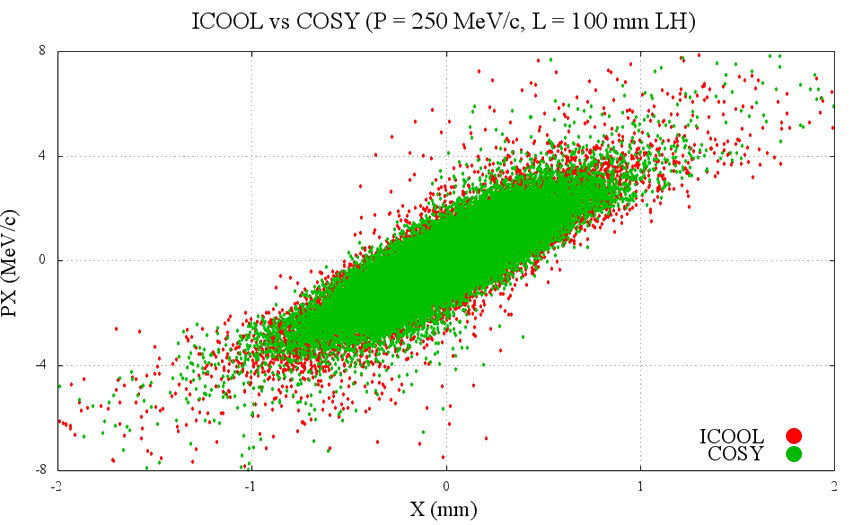
\includegraphics[width=0.7\textwidth]{Figures/xpx_phase_space_implemented} 
  \caption{Sample simulation results for the implementation of the transverse coordinate correction algorithm.}
  \label{fig:xpx_phase_space_implemented}
\end{figure}
%
%-------------------------------------------------------------------------------
%
\Section{Temporal Displacement in COSY Infinity}\label{sec:COSYTemporalDisplacement}\par
For the time-of-flight offset, both the deterministic and stochastic processes are handled in the same routine. To first order, the particle decelerates at some  average rate through an absorber of length $L$. If $a$ is the constant acceleration then 
\begin{align*}
v_f=v_o+a\Delta t,
\end{align*}
or 
\begin{align*}
a=\frac{v_f-v_o}{\Delta t}.
\end{align*}
At the same time, $v_f ^2 = v_o ^2 + 2 a L$, and so
\begin{align*}
 a=\frac{v_f ^2 - v_o ^2}{2L}.
\end{align*}
Then
\begin{align*}
\Delta t = \frac{(v_f-v_o)2L}{v_f^2-v_o^2}.
\end{align*}
Given $\beta=pc/E$ and $v=\beta c$, then
\begin{equation}\label{eqn:cosyDeltaT}
\Delta t=\frac{(\frac{p_f}{E_f}-\frac{p_o}{E_o})2L}{(\frac{p_f ^2}{E_f ^2}-\frac{p_o ^2}{E_o ^2})c^2}.
\end{equation}

However, COSY does not have a time variable, but rather a variable $\ell$ that is described as the time-of-flight in units of length. In COSY \cite{cosy}, this is defined as
\begin{align*}
\ell=\frac{-(t-t_0)v_0\gamma}{1+\gamma},
\end{align*}
where the subscript $0$ signifies the reference particle. Let the time before a step be denoted $t_1$ and the time after a step denoted $t_2$. Then to find $\ell_2$ given $\ell_1$ and $\Delta t$ from Eq. \eqref{eqn:cosyDeltaT}, observe that
\begin{align} \label{eqn:cosyell12}
\begin{split}
\ell_1=\frac{(t_{01}-t_1)v_{01}\gamma_1}{1+\gamma_1} = (t_{01}-t_1)A_1\\
\ell_2=\frac{(t_{02}-t_2)v_{02}\gamma_2}{1+\gamma_2} = (t_{02}-t_2)A_2,
\end{split}
\end{align}
where 
\begin{equation}\label{eqn:cosyAn}
A_n \equiv v_{0n}\gamma_n / (1+\gamma_n) \qquad \text{for }n=1,2.
\end{equation}
Then
\begin{align*}
\ell_2 - \ell_1 &=\big(t_{02}-t_2\big)A_2-(t_{01}-t_1)A_1\\
&=\big([(t_{02}-t_{01})+t_{01}]-[(t_2-t_1)+t_1]\big)A_2-(t_{01}-t_1)A_1\\
&=(\Delta t_0 - \Delta t )A_2 + (t_{01}-t_1)A_2-(t_{01}-t_1)A_2\\
&=(\Delta t_0 - \Delta t )A_2 + (t_{01}-t_1)(A_2-A_1).
\end{align*}
Eq. \eqref{eqn:cosyell12} says that $t_{01}-t_1=\ell_1/A_1$. Moving $\ell_1$ to the right hand side,
\begin{align*}
\ell_2 &= (\Delta t_0 - \Delta t)A_2 + \frac{\ell_1}{A_1}(A_2-A_1)+\ell_1\\
&=(\Delta t_0 - \Delta t)A_2 + \ell_1\Big(\frac{A_2-A_1}{A_1}+\frac{A_1}{A_1}\Big)\\
&=(\Delta t_0 - \Delta t)A_2 + \ell_1\frac{A_2}{A_1}.
\end{align*}
Substituting for $A_n$ via Eq. \eqref{eqn:cosyAn} yields the final result
\begin{equation}\label{eqn:cosyell2}
\ell_2=\frac{(\Delta t_0 - \Delta t) v_{02}\gamma_2}{1+\gamma_2}+\ell_1 \frac{v_{02}\gamma_2 (1+\gamma_1)}{v_{01}\gamma_1 (1+\gamma_2)}.
\end{equation}
Using Eq. \eqref{eqn:cosyell2}, $\Delta t$ from Eq. \eqref{eqn:cosyDeltaT} can be directly input into the new COSY variable for time-of-flight in units of length. Figure~\ref{fig:longitudinal_phase_space} shows the simulation results for a beam of $10^6$ muons of momentum 172 MeV/$c$ passing through 109 mm of liquid hydrogen, which were the parameters of the MuScat experiment \cite{muscat}. The COSY results are shown alongside ICOOL \cite{icool}. Note that the agreement is quite good. ICOOL displays a thicker bulk at around 0.430 ns, but it is approximately 1 ps in width---about 0.2\% of the average time-of-flight.

\begin{figure}[H]
  \centering
    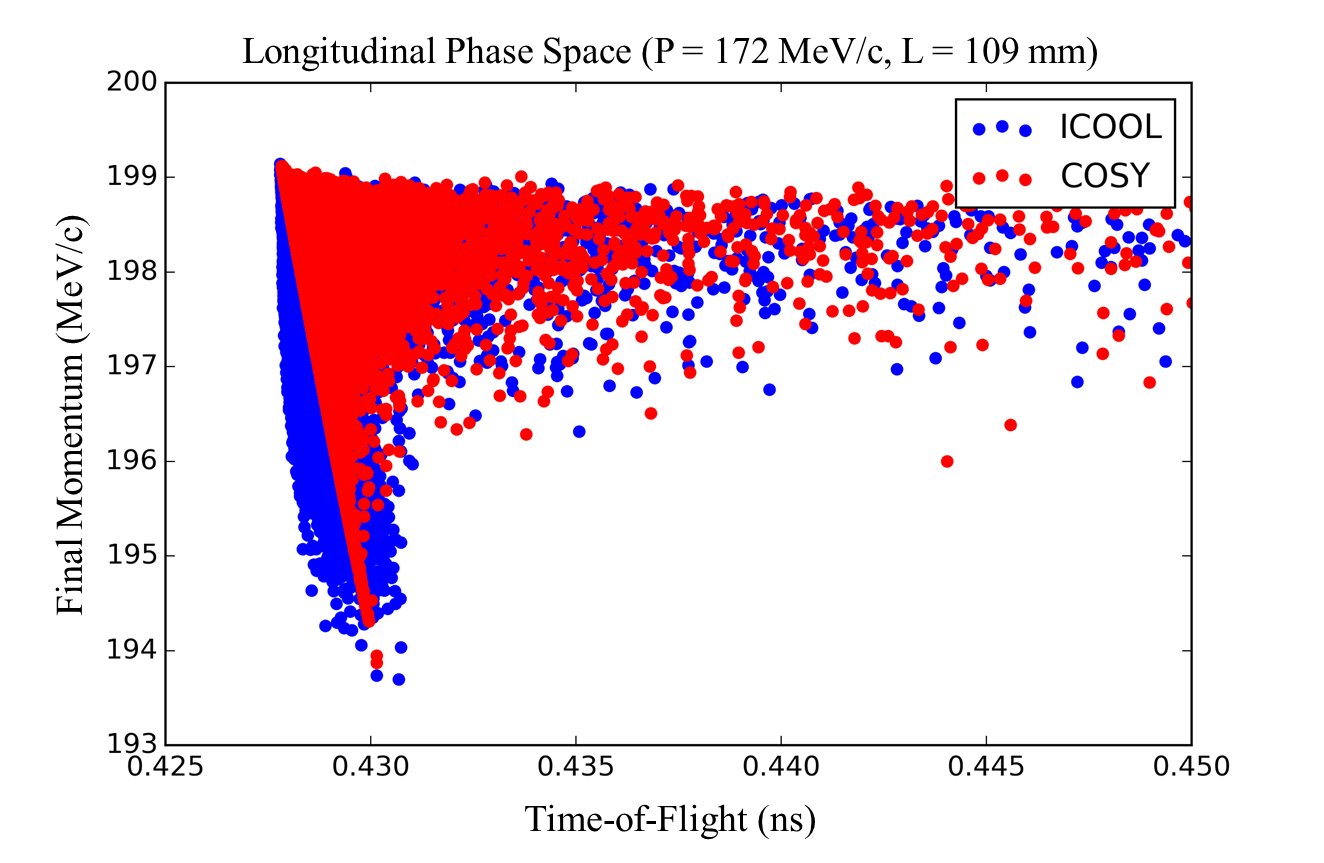
\includegraphics[width=0.7\textwidth]{Figures/longitudinal_phase_space} 
  \caption{Sample simulation results for the implementation of the temporal displacement algorithm discussed in this section.}
  \label{fig:longitudinal_phase_space}
\end{figure}

